\section{Discussion}

% Finding 2: SOT improves meta-learners but not non-meta learners
The most notable finding of our study is the significant role of the SOT module in enhancing the performance of meta-learners, even in challenging few-shot learning scenarios showcasing near-perfect generalisation. However, this performance boost is absent in non-meta learners. This difference likely stems from their distinct training methods. Meta-learners undergo episodic training that mirrors a few-shot environment with support and query samples across classes. The integration of the transductive SOT feature transform module enables optimisation of the backbone with the SOT module enhancing the alignment between support and query samples, crucial for classifying query samples. In contrast, non-meta learners train with random mini-batches and lack a concept of support or query samples. In this setting, the similarity-based feature matrix of the SOT module is meaningless.

% Argument 1) Order matters

% Batch training: 
% - Similarities between samples carry no meaning for multi-class classification problem
% Example: Dog and cat image in 100-way classification problem. Knowledge of cat (doesn't) help predicting dog.

% Episodic training

% During an episode, I am guaranteed to see at least one sample for all classes that I want to predict.
% Hence, matching a query to the closest support is meaningful

A class prediction is independent of all other samples within a batch, making SOT's role in facilitating interaction between support and query samples irrelevant. For instance, in Figure~\ref{fig:sot-embeddings}, the SOT embeddings in the \texttt{PN} model demonstrate clear class-based clustering for both support and query samples, a features less pronounced in the \texttt{B} model.

\begin{figure}[h!]
    \centering
    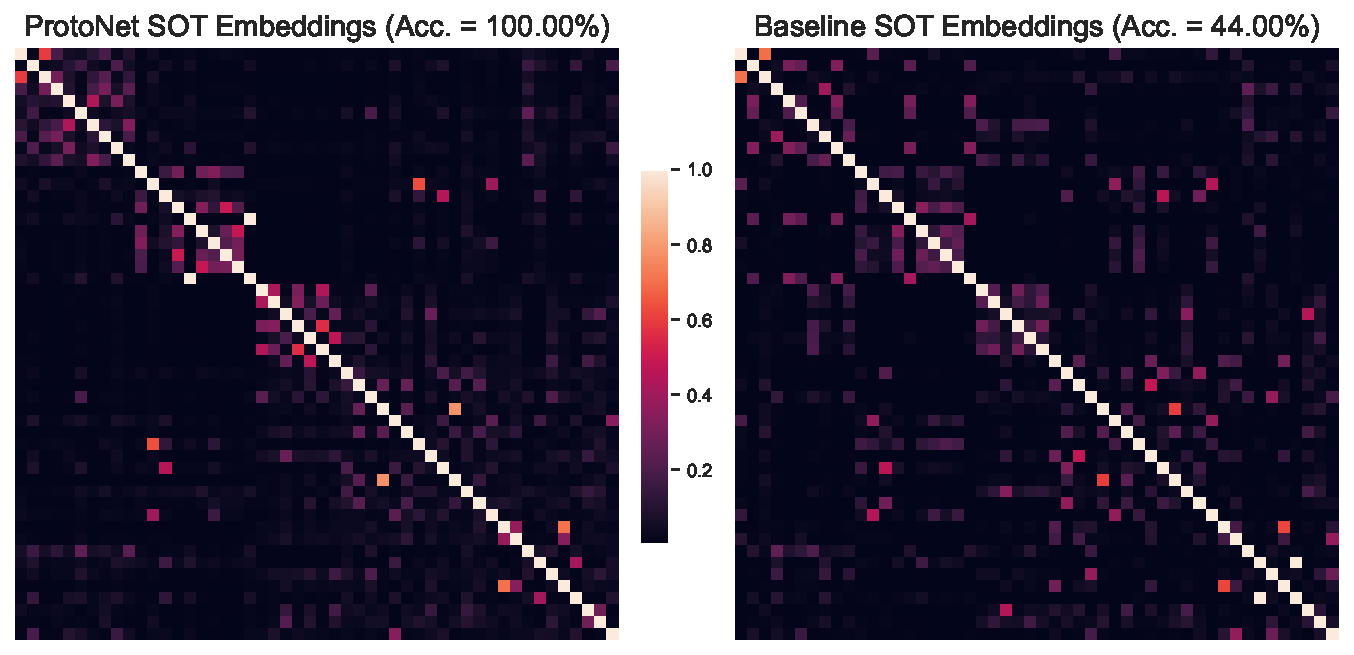
\includegraphics[width=1\columnwidth]{../figures/sot-embeddings.pdf}
    \caption{\textbf{SOT Embeddings.} Heatmap of SOT embeddings for \texttt{PN} (left) and \texttt{B} (right) on the \texttt{SP} dataset for a random test episode in 5-way 5-shot setting. Support and query samples from the same class are adjacent in the embedding matrix.}
    \label{fig:sot-embeddings}
\end{figure}

% Finding 3: SOT improves performance in interaction with LSTM re-embedding
Finally, the ablation study of the re-embedding components in \texttt{MN} suggests that the synergy between the SOT re-embeddings and the LSTM re-embeddings plays a crucial role in the observed performance enhancement of the metric-based meta-learner. The underlying mechanisms of this phenomenon, however, were beyond the purview of this project and are left for future work.
